%label:"fig:FLTZCP2"
%author:JeffHicks
%name:"the FLTZ skeleton given by the fan for CP2"
%type:"figure"
%parent:"exm:FLTZSkeletonCP2"
%caption:"the FLTZ skeleton for the fan for $\mathbb {CP}^2$. "

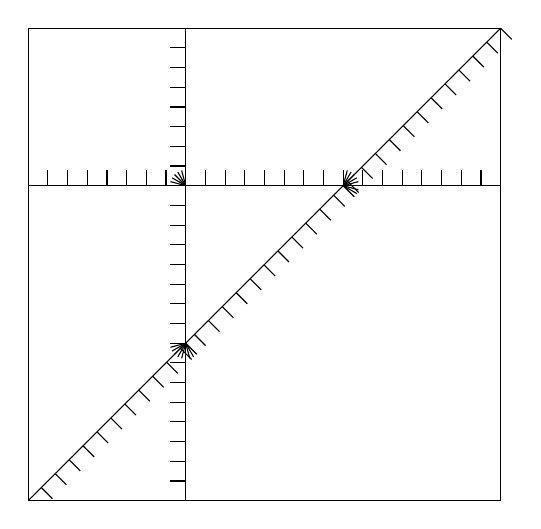
\begin{tikzpicture}
    \tikzstyle{fuzz}=[
        postaction={draw, decorate, decoration={border, amplitude=0.2cm,angle=90 ,segment length=.25cm}},
    ]
    
       
    \draw[fuzz] (-5,1) -- (1,1);
    \draw  (-5,3) rectangle (1,-3);
    \draw[fuzz] (-3,-3) -- (-3,3);
    \draw[fuzz] (1,3) -- (-5,-3);
    
    
    
    
    \begin{scope}[shift={(-3,1)}]
    \foreach \i in {6,...,12}
    {
            \pgfmathtruncatemacro{\y}{15* \i };
            \draw (0,0)-- (\y:.2) ;
    }
    
    \node at (0,0) {};
    \end{scope}
    
    
    \begin{scope}[shift={(-3,-1)}]
    \foreach \i in {12,...,21}
    {
            \pgfmathtruncatemacro{\y}{15* \i };
            \draw (0,0)-- (\y:.2) ;
    }
    
    \node at (0,0) {};
    \end{scope}
    
    
    
    \begin{scope}[shift={(-1,1)}]
    \foreach \i in {-3,...,6}
    {
            \pgfmathtruncatemacro{\y}{15* \i };
            \draw (0,0)-- (\y:.2) ;
    }
    
    \node at (0,0) {};
    \end{scope}
    
\end{tikzpicture}